\glsreset{de}
\glsreset{ea}
\chapter{Der Lösungsansatz}
\label{chap:sol}

	Dieses Kapitel beginnt mit einer Einführung in die Evolutionären Algorithmen und stellt daraus exemplarisch die Differentielle Evolution vor. Zum Schluss dieses Kapitels folgt eine Einbindung der Differentiellen Evolution in den Kontext der Segmentierung.

	\section{\gls{ea}}
	\label{sec:evol}
	
		Hierbei handelt es sich, wie in \cite{ea-intro} beschrieben, um heuristische Verfahren zur Lösung von Problemen, die andernfalls nicht in polynomialer Zeit gelöst werden können. Dabei orientieren sie sich an den Vorgängen der biologischen Evolution. Die Begründung hierfür wird von John H. Holland (gefunden in \cite{ger-kla-kru-intro}) in prägnanter Weise dargelegt: 
	
		\begin{quote}
			\textit{Lebewesen sind vollendete Problemlöser. In der Vielzahl der Aufgaben, die sie bewältigen, übertreffen sie die besten Computerprogramme bei weitem - zur besonderen Frustration der Programmierer, die Monate oder gar Jahre harter geistiger Arbeit für einen Algorithmus aufwenden, während Organismen ihre Fähigkeiten durch den scheinbar ziellosen Mechanismus der Evolution erwerben.}
		\end{quote}
	
		Dieses Zitat bietet eine grobe Vorstellung vom Wesen und der Herkunft von \gls{ea}. In vielen literarischen Werken zu diesem Thema - beispielsweise \cite{ger-kla-kru-intro, eib-smi-ea} - wird festgehalten, dass verschiedene Kategorien von \gls{ea}s existieren. Allerdings ist die zugrunde liegende Idee hinter all diesen Sorten von Algorithmen die selbe und wird von den Autoren in \cite{eib-smi-ea} wie folgt dargelegt:\\
		Gegeben sei eine Gruppe von Individuen, genannt \textit{Population}, die innerhalb einer Umgebung mit begrenzten Ressourcen lebt. Der Kampf um diese löst eine natürliche Selektion aus und führt so zu einer höheren Fitness der Population - ein Vorgang, der sehr gut unter dem Stichwort \textit{Survival of the Fittest} bekannt ist. Nach diesem Vorbild aus der Natur nehme man
		\begin{itemize}
			\item ein zu lösendes Problem (stellvertretend für die Umgebung), abgebildet durch eine (Fitness-)Funktion, die maximiert oder minimiert werden soll, sowie
			\item eine Menge an Lösungskandidaten (im Folgenden als Individuen bezeichnet), bestehend aus einem Set von Funktionsparameterlisten.
		\end{itemize}
		Auf diese Individuen wird sodann die Fitnessfunktion angewendet und mit dem Ergebnis in abstrakter Weise jeweils die Fitness der einzelnen Individuen gemessen. Dabei erfolgt die Bewertung abhängig davon, ob minimiert oder maximiert werden soll. Im folgenden Schritt erzeugen verschiedene Variationsoperatoren wie Mutation und/oder Rekombination aus der Ursprungspopulation eine neue Population, für die wiederum die Fitnessfunktion ausgewertet wird. Auf der Basis der jeweiligen Fitnesswerte werden die korrespondierenden Individuen beider Populationen verglichen und davon dasjenige mit der höheren Fitness in die Population der nächsten Generation übernommen.
	
		Die oben genannten Schritte werden so lange iteriert, bis entweder eine geeignete Lösung gefunden wurde oder eine (vorher definierte) maximale Anzahl an Iterationen erreicht ist. Abbildung \ref{fig:ea-flowchart}. veranschaulicht die Funktionsweise von \gls{ea}s nochmals in Form eines einfachen Flussdiagramms.
	
		\begin{figure}[h]
			\centering
			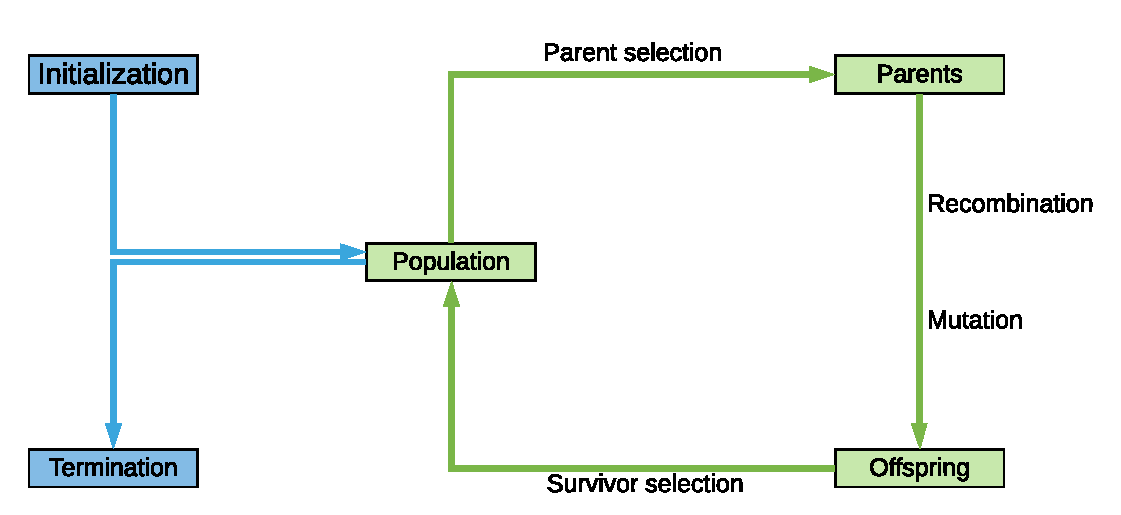
\includegraphics[width=\linewidth]{ea_flowchart}
			\caption[Genereller Ablauf von \gls{ea}s]{Genereller Ablauf von \gls{ea}s (Nachbildung der Graphik aus \cite[Seite 27]{eib-smi-ea})}
			\label{fig:ea-flowchart}
		\end{figure}
	
		Nachstehend wird in Abschnitt \ref{sec:de} die Methode der 
		\textit{Differentiellen Evolution} als Beispiel vorgestellt und in den 
		weiteren Kontext der vorliegenden Arbeit eingebettet.
	
		\glsreset{de}

	\section{\gls{de}}
	\label{sec:de}

		Die Autoren in \cite{storn-price-de} entwickelten diese Methode mit Hinblick auf die im Anschluss gelisteten Anforderungen an ein in der Praxis anwendbares Optimierungsverfahren:
		\begin{enumerate}
			\item Es soll mit nicht-differenzierbaren und nicht-linearen 
			Funktionen, die unter Umständen mehrere (lokale) Maxima/Minima 
			aufweisen, umgehen können.
			\item Falls eine sehr rechenintensive Funktion auftritt, soll das 
			Verfahren parallelisierbar sein. Es soll also möglich sein, die 
			Berechnungen auf mehrere Prozessorkerne auszulagern.
			\item Weiterhin soll die Methode leicht zu benutzen sein. Im 
			gegebenen Kontext bedeutet dies zum Beispiel, dass sie wenige 
			Kontrollparameter besitzt, die einfach bestimmbar sind.
			\item Außerdem soll sie sich mit steigender Iterationszahl immer 
			näher dem \textbf{globalen} Minimum/Maximum annähern.
		\end{enumerate}
		Zwar ist \gls{de} laut \cite{storn-price-de} darauf ausgerichtet, die 
		oben genannten Bedingungen zu erfüllen, den Wahrheitsgehalt dieser 
		Aussage zu prüfen soll jedoch nicht Aufgabe der hier vorliegenden 
		Arbeit sein. Hier liegt der Fokus primär auf der Anwendung des 
		Verfahrens mit der Annahme, die vorangestellte Aussage sei wahr.\\
		
		Der nachstehende Pseudocode beschreibt die substanzielle Idee hinter \gls{de} in etwas vereinfachter Form \cite[S. 34]{storn-price-de-book}:\\
		
		\begin{algorithm*}[H]
			\SetAlgoLined
			...\\
			while(convergence criterion not yet met)\{
				\begin{tabbing}
					Links \= Mitte \= Rechts \= WeiterRechts \kill
					\>//---$x_{i}$ defines a vector of the current vector population-------\\
					\>//---$y_{i}$ defines a vector of the new vector population-----------\\
				
					\>for ($i=0$; $i<N_{p}$; i++) \{\\
				
					\>\>$r_{1} = rand(N_{p});$ //select a random index from $1, 2, ..., N_{p}$\\
					\>\>$r_{2} = rand(N_{p});$ //select a random index from $1, 2, ..., N_{p}$\\
					\>\>$r_{3} = rand(N_{p});$ //select a random index from $1, 2, ..., N_{p}$\\
					\>\>\textbf{$u_{i} = x_{r_{3}} + F * (x_{r_{1}} - x_{r_{2}})$};\\
					\>\>if $f(u_{i}) \leq f(x_{i})$  then \{\\
						\>\>\>$y_{i} = u_{i};$\\
					\>\>\} else \{\\
						\>\>\>$y_{i} = x_{i};$\\
					\>\>\}\\
					\>\}
				\end{tabbing}
			\}
			...
			
		\end{algorithm*}
		\begin{center}
			\TitleOfAlgo{Pseudo-Code für \gls{de}}
		\end{center}
		
	
		mit $N_{p}$ für die Größe der Population stehend.\\
		Mit der Zeit haben sich unterschiedliche Varianten von \gls{de} herausgebildet. Die gängige Notation hierfür folgt dem Schema \textit{\gls{de}/x/y/z}, wobei sich die Bedeutung der Variablen x, y und z im Verlauf der nachfolgenden detaillierten Beschreibung der einzelnen Operationen in \gls{de} an geeigneter Stelle erschließen werden \cite{storn-price-de, storn-price-de-book}: 
		%\vfill
		
		\subsection{Initialisierung}
		\label{sub:de-init}
		
			Zunächst muss die initiale Population $P_{0}$ mit ihren Mitgliedsvektoren $x_{i, 0}$ erzeugt werden. Hier hat sich die Verwendung von gleich-verteilt angenommenen Zufallszahlen bewährt. Um den Bezug zur jeweiligen Anwendung herzustellen, müssen zu den zufälligen Werten sinnvolle Ober-und Untergrenzen $b_{j, U}$ und $b_{j, L}$ angegeben werden, sodass die Vektorelemente $x_{j, i, 0}$ nach folgendem Zusammenhang errechnet werden:
			\begin{flalign}
				x_{j, i, 0} = rand(0,1) \cdot (b_{j, U} - b_{j, L}) + b_{j, L}, \quad j = 1, 2, ..., Dim(x_{i, 0}) \label{eq:de-init}
			\end{flalign}  
			
		\subsection{Mutation}
		\label{sub:de-mutation}
		
			Für alle $x_{i, g}$ werden Mutantenvektoren $v_{i, g}$ gebildet, indem zu einem ausgewählten Basisvektor aus der gegenwärtigen Population gemäß der Gleichung \ref{eq:de-mutation} die skalierte Differenz zweier zufällig gewählter, voneinander verschiedener Vektoren addiert wird: 
			\begin{flalign}
				v_{i, g} = x_{r_{0}} + F \cdot (x_{r_{1}, g} - x_{r_{2}, g}) \label{eq:de-mutation}
			\end{flalign}
			Der Faktor $F \in (0,\infty($ beeinflusst die Rate der Mutation. Theoretisch gibt es für $F$ keine obere Schranke, aber in der Praxis haben sich Werte im Bereich $(0,2)$ bewährt.\\
			Für die Auswahl des Index $r_{0}$ gibt es unterschiedliche Möglichkeiten, abhängig vom konkreten Algorithmus. Im Fall der klassischen \gls{de}-Variante \gls{de}/\textbf{rand}/1/bin
			ist $r_{0}$ ein weiterer zufällig ausgewählter Index ungleich $r_{1}$ und $r_{2}$. Dahingegen wird $r_{0}$ bei dem in \cite{cuevas-meth1} und auch in dieser Arbeit verwendeten Algorithmus \gls{de}/\textbf{best}/1/exp zum Index desjenigen Vektors $x$, für den $f(x)$ innerhalb der aktuellen Population den kleinsten/größten Wert zurückgibt. Die \textbf{1} bei der Algorithmen-Kennzeichung gibt im Übrigen an, dass ein einziger Differenzvektor gebraucht wird - so in Gleichung \ref{eq:de-mutation} zu sehen.
		\subsection{Crossover}
		\label{sub:de-crossover}
		
			Das Ergebnis der Crossover-Operation ist eine neue Population, die 
			beim Selektionsvorgang in Paragraph \ref{sub:de-selection} mit der 
			Ursprungspopulation konkurriert, mit den Vektoren $u_{i, g}$ und 
			ihren Parametern $u_{j, i, g}$ mit $j = 1, 2, ... , D$. Deren 
			Ermittlung kann ebenfalls je nach Abwandlung von \gls{de} 
			unterschiedliche Formen annehmen: \\
			Im Vergleich dazu wird hier der \textit{Exponentielle Crossover} benutzt. Der folgende Pseudo-Code veranschaulicht dessen Funktionsweise:\\
			\begin{algorithm*}[H]
				\SetAlgoLined
				$j_{r} = \textrm{floor}(\textrm{rand}(0,1) \cdot D);$ // $0 \leq j_{r} < D$\\
				$j = j_{r};$\\
				do \{
				\begin{tabbing}
					Links \= Mitte \= Rechts \kill
					\>$u_{j,i} = v_{j,i};$ \qquad // Child inherits a mutant parameter\\
					\>$j = (j+1) \% D;$ \qquad // Increment j, modulo D 
				\end{tabbing}
				\}while($\textrm{rand}(0,1) < C_{r} \ \&\& \ j \neq j_{r}$); // Take another mutant parameter?\\
				while($j \neq j_{r}$) \{
				\begin{tabbing}
					Links \= Mitte \= Rechts \kill
					\>$u_{j,i} = x_{j,i};$ \\
					\>$j = (j+1) \% D;$ \}
				\end{tabbing}
			\end{algorithm*}
			\begin{center}
				\TitleOfAlgo{Pseudo-Code für exponentiellen Crossover \cite[S. 94]{storn-price-de-book}}
			\end{center}
			
			Bei der klassischen Version (\gls{de}/rand/1/\textbf{bin}) kommt der \textit{Binomiale Crossover} zum Einsatz. Hierbei wird mit der Bestimmung eines zufälligen Parameterindex $j_{rand} \in \{1,2,...,D\}$ begonnen. Damit werden die Elemente $u_{j, i, g}$ zu
			\begin{flalign}
				\centering
				u_{j, i, g} = 
				\begin{cases}
				v_{j, i, g} \quad \textrm{if}(\textrm{rand}(j) \leq C_{r}) \textrm{ or } j = j_{rand} \\
				x_{j, i, g} \quad \textrm{if}(\textrm{rand}(j) > C_{r}) \textrm{ and } j \neq j_{rand}
				\end{cases}
				\label{eq:de-bin-cross}
			\end{flalign}
			mit $\textrm{rand}(j)$ als j-te Ziehung aus einer gleichverteilten Menge von Zufallszahlen und $C_{r}$ als Crossover-Konstante, die die Anzahl an Parametern, die vom Mutationsvektor $v_{i}$ kommen, beeinflusst.
			
		\subsection{Selektion}
		\label{sub:de-selection}
			Zum Schluss werden die Populationsmitglieder der nächsten Generation aus der vorherigen Population $x$ und der Versuchspopulation $u$ selektiert. Als Auswahlkriterium wird $f(x_{i})$ bzw. $f(u_{i})$ herangezogen:
			\begin{flalign}
				x_{i, g+1} = 
				\begin{cases}
					u_{i, g} \ \textrm{if } f(u_{i,g}) \leq f(x_{i,g}) \ \textrm{(min), } \quad f(u_{i,g}) \geq f(x_{i,g}) \ \textrm{(max)} \\
					x_{i,g} \ \textrm{sonst}
				\end{cases}
			\end{flalign}
			
	\section{Zusammenführung von Differenzieller Evolution und Segmentierung}
	\label{sec:diff-seg-together}
		
		\subsection{Modell 1}
		\label{sub:model1}
			Wie bereits in Paragraph \ref{sub:meth1} angekündigt worden ist, soll \gls{de} dazu benutzt werden, das dort gestellte Optimierungsproblem zu lösen. Dazu werden die für \gls{de} relevanten Sachverhalte wie folgt definiert:\\
			Die zu optimierende Funktion $f(x)$ ist in diesem Fall gegeben durch den mittleren quadratischen Fehler $E$, für den die $D = 3K$ Parameter $\sigma_{i}$, $\mu_{i}$ und $P_{i}$ derart bestimmt werden müssen, dass das in Gleichung \ref{eq:mean-square-error} aufgestellte Problem möglichst gut gelöst wird. Da $K \geq 2$ gilt - denn jeder Wert darunter ist im Kontext einer Segmentierung sinnbefreit - beläuft sich die Größe $D$ der Populationsvektoren $x_{i}$ auf wenigstens 6. Wird zusätzlich die Populationsgröße $N_{p}$ mit einbezogen, beläuft sich die Gesamtzahl der Elemente auf $N_{p} \cdot D$, sodass die Population aus $N_{p}$ Vektoren der Form $x_{i} = \{\sigma_{1}, \mu_{1}, P_{1}, ..., \sigma_{K}, \mu_{K}, P_{K}\}$ besteht.
			
		\subsection{Modell 2}
		\label{sub:model2}
			Auch hier soll aus Gründen der Nachvollziehbarkeit die Verknüpfung zwischen \gls{de} und dem K-Means-Clusterverfahren hergestellt werden. Hier ist $f(x)$ gegeben durch die Summe der euklidischen Distanzen aller Pixel $p_{i}$ zu jedem Segment-Mittelpunkt $\mu_{1}$ in Gleichung \ref{eq:kmeans-min}. Das dortige Optimierungsproblem ist so formuliert, dass eine Segmentierung $S = \{\mu_{1}, ..., \mu_{K}\}$ gesucht ist, die jene im vorigen Satz genannte Summe möglichst klein werden lässt. Demzufolge entsprechen die Segmentierungen $S$ in diesem Fall genau den Populationsmitgliedern $x_{i}$, womit die Zahl der Elemente zu $N_{p} \cdot K$ wird.\\
			Es sei angemerkt, dass bei der Berechnung der Mittelpunkte $\mu_{i}$ sowohl der \textit{Assignment-}Step als auch der \textit{Update}-Step wegfallen, da jene durch die Operatoren des \gls{de}-Algorithmus kalkuliert werden. Lediglich der erste von beiden Schritten wird bei der Segmentierung schließlich ausgewertet.